
%\todo{Start here. 4 pages each and 2 pages discussion. Target 20 pages.}

%msection{Generating Software Diversification for WebAssembly}
Generating  WebAssembly binaries is a process that commences with the original source code.
This code is processed by a compiler, which can be conceptually divided into three primary components: a front-end that translates the source code into an intermediate representation, an optimizer that transforms this representation for the sake of performance, and a back-end that assembles the final \Wasm binary. 
This modular architecture is perfectly implemented by LLVM, a compiler framework that supports a wide array of programming languages, including C, C++, and Rust. 

Software Diversification, a proactive security measure, can be integrated at different points along this compilation pipeline. 
Yet, this strategy is limited if applied to the front-end. 
Specifically, it would need the development of a unique diversification mechanism for each language that can be compiled into \Wasm, rendering it impractical for widespread use. 
For instance, in the case of LLVM, one would need to modify each of the front-ends to introduce diversification. 
Yet, implementing diversification at later stages of the compiler, such as the optimizer or the back-end, presents a more viable alternative. 
This is especially important given that approximately 70\% of \Wasm binaries are produced using LLVM-based compilers, as indicated by Hilbig et al. \cite{Hilbig2021AnES}.
Therefore, featuring diversification techniques in the latter compiler stages is viable, leading us to propose compiler-based approaches to diversify \Wasm binaries. 


\begin{figure}[h]
	\centering
	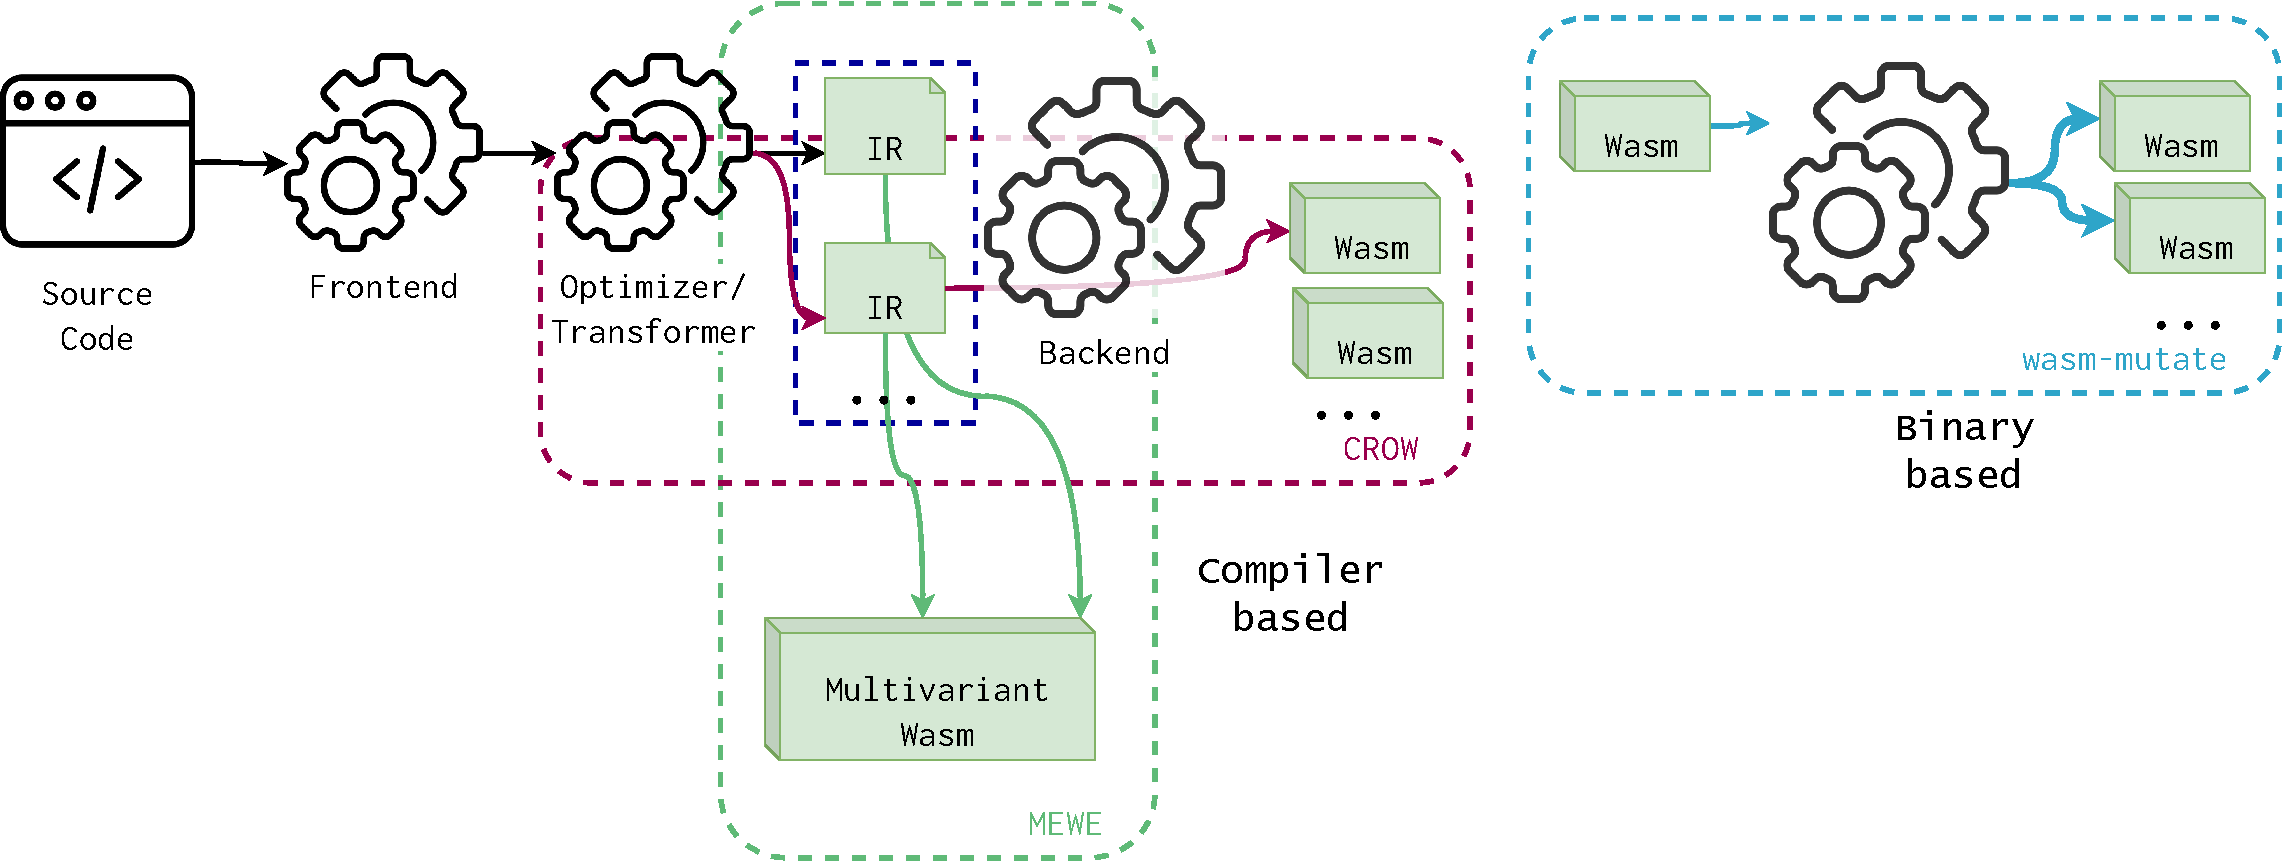
\includegraphics[width=1.0\textwidth]{figures/landscape.pdf}
	\caption{Approach landscape containing our three technical contributions: CROW squared in red, MEWE squared in green and WASM-MUTATE squared in blue. We annotate where our contributions, compiler-based and binary-based, stand in the landscape of generating \Wasm programs.}
	\label{fig:approach_landscape}
\end{figure}

% Compiler based approaches
Our compiler-based strategies are highlighted in red and green in \autoref{fig:approach_landscape}. 
This approach introduces a diversifier component in the LLVM pipeline, generating LLVM IR variants and producing artificial software diversity for \wasm. 
This strategy encompasses two tools: CROW \cite{CROW}, which creates \wasm program variants, and MEWE \cite{MEWE}, which merges these variants to provide multivariant execution \cite{cox06} for \wasm.


On the other hand, diversification can be directly applied to the \Wasm binary.
This offers the most flexible approach since it is agnostic to the original programming language or the compiler employed.
We propose a binary-based approach, WASM-MUTATE, which is illustrated in blue in \autoref{fig:approach_landscape}.
WASM-MUTATE \cite{wasmmutate} generates a pool of \Wasm program variants through rewriting rules upon an e-graph \cite{e-graph} data structure.


To sum up, this dissertation contributes to the field of Software Diversification for \Wasm through two strategies: compiler-based and binary-based.
We present three main technical contributions: CROW, MEWE, and WASM-MUTATE, dissected upon in the subsequent sections.
Moreover, we compare our technical contributions between them, showcasing that they are complementary and can be used in conjunction to provide a more robust diversification strategy.
Furthermore, we outline the artifacts for our three technical contributions for the sake of open-research and reproducibility.

